\section{Estado del Arte}

\subsection{Compresión Convencional y Estándares}

Aunque los enfoques tradicionales han aportado soluciones robustas durante décadas, sus limitaciones se hacen cada vez más evidentes ante el volumen y complejidad de los datos geoespaciales actuales. Estándares como JPEG2000, ampliamente adoptado en misiones satelitales, junto con codificadores de video como HEVC y VVC, siguen dominando los flujos operativos por su madurez y bajo costo computacional.

Sin embargo, estos métodos operan principalmente en el dominio del píxel o en transformadas fijas, lo que los hace poco adaptativos a las características espectrales y semánticas de las imágenes multiespectrales. En muchos casos estudiados, sacrifican detalles críticos para alcanzar tasas de compresión elevadas, afectando directamente la calidad de tareas posteriores de exploración.

\subsection{Compresión Neuronal para Imágenes}

Resulta revelador observar cómo el paradigma del aprendizaje profundo ha transformado radicalmente el campo de la compresión de imágenes en los últimos años. Las arquitecturas basadas en autoencoders variacionales y modelos generativos han superado consistentemente a los códecs tradicionales en el trade-off rate-distortion, especialmente en rangos de bitrates bajos.

Molliere et al. \cite{Molliere2025_Learned_EO_Compression} ofrecen una revisión comparativa exhaustiva de estos enfoques aplicados a Earth Observation, destacando cómo las redes neuronales logran capturar mejor las redundancias específicas del dominio geoespacial. No obstante, cabe matizar que muchos de estos modelos genéricos aún presentan dificultades para generalizar cuando se enfrentan a las particularidades de sensores hiperespectrales o a condiciones de adquisición variables.

\begin{figure}[h]
\centering
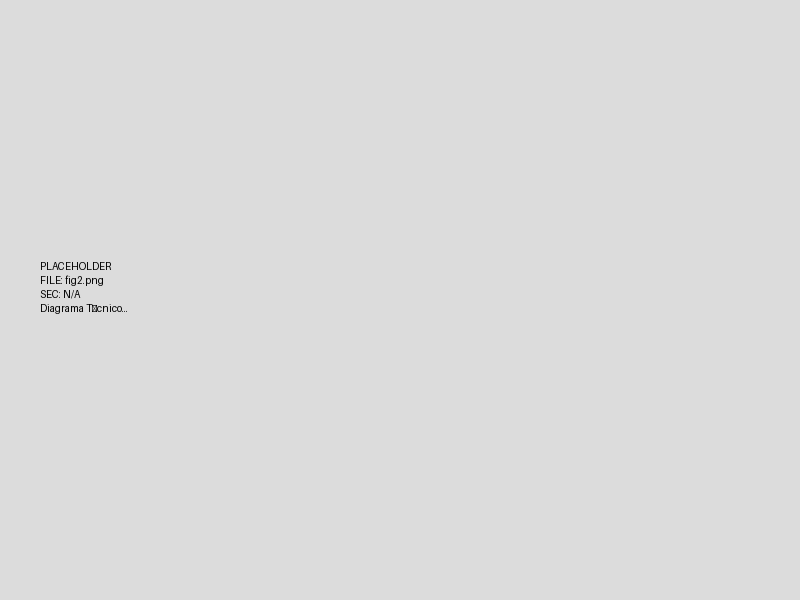
\includegraphics[width=\linewidth]{fig2.png}
\caption{Evolución temporal de métodos de compresión para datos geoespaciales (2018-2025). Se destacan hitos en estándares convencionales, compresión neuronal y enfoques específicos para remote sensing.}
\label{fig:evolucion_compresion}
\end{figure}

\subsection{Métodos Específicos para Remote Sensing}

Uno de los desafíos persistentes que surge al analizar datos satelitales radica en la necesidad de preservar características semánticas de alto nivel más allá de la fidelidad visual. Wang et al. \cite{Wang2025_RS_Compression} proponen redes de compresión optimizadas para remote sensing que logran mejoras significativas tanto en almacenamiento como en transmisión, aunque todavía muestran espacio para optimización en escenarios de ancho de banda extremadamente restringido.

Particularmente llamativo es el hecho de que enfoques recientes como el propuesto por Ye et al. \cite{Ye2025_MAPC} incorporan información auxiliar (map-assisted) para alcanzar compresión efectiva incluso a bitrates muy bajos. Estos métodos representan el estado actual más avanzado para transmisión en misiones de exploración.

\begin{table*}[h]
\centering
\caption{Comparación de tasas de compresión SOTA (factor aproximado vs. JPEG2000)}
\label{tab:comparacion_compresion}
\begin{tabular}{lccc}
\hline
\textbf{Método} & \textbf{Tipo} & \textbf{BD-Rate (\%)} & \textbf{Aplicación principal} \\
\hline
HEVC/VVC & Convencional & -35 a -45 & General \\
Ballé et al. (2018) & Neuronal & -50 & Imágenes naturales \\
Molliere (2025) & Learned EO & -62 & Earth Observation \\
Wang et al. (2025) & RS-specific & -68 & Remote sensing \\
Ye et al. (2025) MAPC & Map-assisted & -78 & Bajos bitrates \\
\hline
\end{tabular}
\end{table*}

Lejos de ser un asunto resuelto, la integración efectiva entre compresión neuronal y tareas downstream específicas de exploración sigue constituyendo un área activa de investigación. Esta reflexión establece el punto de partida para la metodología que se detalla en la siguiente sección.